\chapter{कमान में मस्तिष्क}\label{ch:g5:brain-in-command}

एक गेंद तुम्हारी ओर उड़ती है; तुम उसे लपक लेते हो। आधा सेकंड, और सोच
बिलकुल नहीं --- फिर भी उस आधे सेकंड में तुम्हारी \omterm{def:g1:the-five-senses:sense}{आँखों} ने एक उड़ती चीज़
की ख़बर दी, किसी ने उसका रास्ता निकाला, और दर्जनों \omterm{def:g3:bones-and-muscles:muscle}{पेशियों} को ठीक-ठीक
सही लपक का आदेश मिला। वह ``कोई'' \omterm{def:g5:brain-in-command:system}{मस्तिष्क} है, और यह अध्याय शरीर की
तारों पर उसके आदेशों के पीछे चलता है।

\section{कमान का जाल}

\begin{definition}[तंत्रिका तंत्र]\label{def:g5:brain-in-command:system}
\emph{तंत्रिका तंत्र}\index{तंत्रिका तंत्र} शरीर का कमान-जाल है:
\begin{itemize}
  \item \emph{मस्तिष्क}\index{मस्तिष्क}, जो \omterm{def:g3:bones-and-muscles:skeleton}{खोपड़ी} की ओट में रहता है
        (\cref{def:g3:bones-and-muscles:skeleton}), केंद्र है: वह
        सारी ख़बरें पाता है और सारे आदेश जारी करता है;
  \item \emph{मेरुरज्जु}\index{मेरुरज्जु}, तंत्रिका ऊतक की एक मोटी
        रस्सी, मस्तिष्क से नीचे \omterm{def:g4:classifying-animals:vertebrate}{रीढ़} के रक्षक खंभे के भीतर चलती है;
  \item \emph{तंत्रिकाएँ}\index{तंत्रिका}, यानी सफ़ेद धागे, जो
        मस्तिष्क और मेरुरज्जु से निकलकर हर अंग तक जाते हैं और संदेश
        ढोते हैं --- सबसे तेज़ तो \qty{100}{m/s} से भी ऊपर।
\end{itemize}
\end{definition}

\begin{proposition}[ख़बर, फ़ैसला, आदेश]\label{prop:g5:brain-in-command:loop}
हर क्रिया एक ही घेरे पर चलती है
(\cref{prop:g1:the-five-senses:brain} उसका पहला ख़ाका था):
\begin{enumerate}
  \item \emph{ज्ञानेंद्रियाँ} ख़बर देती हैं: \omterm{def:g5:brain-in-command:system}{तंत्रिकाएँ} उनके संदेश
        \omterm{def:g5:brain-in-command:system}{मस्तिष्क} \emph{तक} ले जाती हैं;
  \item \emph{\omterm{def:g5:brain-in-command:system}{मस्तिष्क}} ख़बरों को जोड़ता है, फ़ैसला करता है, और आदेश
        गढ़ता है;
  \item \omterm{def:g5:brain-in-command:system}{तंत्रिकाएँ} वे आदेश \omterm{def:g5:brain-in-command:system}{मस्तिष्क} \emph{से} \emph{\omterm{def:g3:bones-and-muscles:muscle}{पेशियों}} तक ले
        जाती हैं (\cref{def:g3:bones-and-muscles:muscle}), और वे आदेश
        पर \omterm{def:g3:bones-and-muscles:muscle}{संकुचित} हो जाती हैं।
\end{enumerate}
ज्ञानेंद्रियाँ ख़बर देती हैं, \omterm{def:g3:bones-and-muscles:muscle}{पेशियाँ} मानती हैं --- फ़ैसला कोई नहीं करता।
\end{proposition}
\admitted

\begin{omfigure}
\begin{tikzpicture}
  % eye
  \draw[thick] (-0.7,1.7) ellipse (0.5 and 0.28);
  \fill[omDef] (-0.58,1.7) circle (0.13);
  \node[font=\small, align=center] (eye) at (-0.7,0.85)
    {आँख गेंद\\ देखती है};
  % brain
  \draw[thick, omDef, fill=omDef!8, rounded corners=8pt]
    (3.2,1.15) rectangle (6.4,2.45);
  \node[font=\small\bfseries, omDef] at (4.8,2.05) {मस्तिष्क};
  \node[font=\footnotesize] at (4.8,1.55) {लपक का फ़ैसला करता है};
  % muscle
  \draw[thick, omThm, fill=omThm!15]
    (9.6,1.5) .. controls (10.0,1.85) and (10.6,1.85) .. (11.0,1.55)
    .. controls (10.6,1.35) and (10.0,1.35) .. (9.6,1.5);
  \node[font=\small, align=center] at (10.3,0.85)
    {बाँह की पेशियाँ\\ संकुचित होती हैं};
  % arrows
  \draw[->, very thick, omMeth] (-0.1,1.7) -- (3.1,1.8)
    node[pos=0.42, above=2pt, font=\footnotesize, omMeth]
    {ख़बर, तंत्रिका के रास्ते};
  \draw[->, very thick, omProp] (6.5,1.8) -- (9.5,1.6)
    node[pos=0.5, above=2pt, font=\footnotesize, omProp]
    {आदेश, तंत्रिका के रास्ते};
\end{tikzpicture}

{\small हर क्रिया का घेरा: \omterm{def:g5:brain-in-command:system}{मस्तिष्क} तक ख़बर, फ़ैसला, और \omterm{def:g3:bones-and-muscles:muscle}{पेशियों} तक
आदेश।}
\end{omfigure}

\begin{example}[लपक, धीरे-धीरे दोहराई हुई]\label{ex:g5:brain-in-command:catch}
उस आधे सेकंड को फिर से चलाओ: \omterm{def:g1:the-five-senses:sense}{आँखें} गेंद पर नज़र रखती हैं और लगातार
ख़बर देती हैं; \omterm{def:g5:brain-in-command:system}{मस्तिष्क} ख़बर दर ख़बर मिलाकर निकालता है कि गेंद कहाँ
होगी; और आदेश \omterm{def:g1:my-body:parts}{टाँगों} (एक क़दम बाएँ), \omterm{def:g1:my-body:parts}{धड़} (झुको), \omterm{def:g1:my-body:parts}{बाँह} तथा उँगलियों
(खोलो --- अब बंद करो) तक बहते जाते हैं। किसी एक अंग ने ``गेंद नहीं
लपकी'': \omterm{def:g1:the-five-senses:sense}{आँखों}, \omterm{def:g5:brain-in-command:system}{मस्तिष्क} और \omterm{def:g3:bones-and-muscles:muscle}{पेशियों} में से हर एक ने
\cref{prop:g5:brain-in-command:loop} की अपनी पंक्ति निभाई।
\end{example}

\begin{remark}[सिर्फ़ हरकत नहीं]\label{rem:g5:brain-in-command:more}
जो \omterm{def:g5:brain-in-command:system}{मस्तिष्क} गेंदें लपकता है, वही तुम्हारी यादें भी रखता है, इस पन्ने
पर तुम्हारा ध्यान थामे रहता है, रात में सपने देखता है --- और वे सेवाएँ
भी चलाता है जिनके बारे में तुम कभी सोचते तक नहीं: वह दिन-रात साँस चलती
रखता है (\cref{def:g4:breathing:movements}) और शरीर की ज़रूरत के
हिसाब से \omterm{def:g4:heart-and-blood:heart}{हृदय} की चाल बदलता रहता है
(\cref{ex:g4:heart-and-blood:effort})। कुछ आदेश तुम्हें देने होते हैं;
बाक़ी \omterm{def:g5:brain-in-command:system}{मस्तिष्क} तुम्हारे लिए दे देता है।
\end{remark}

\section{घेरे को नापना: प्रतिक्रिया काल}

\begin{definition}[प्रतिक्रिया काल]\label{def:g5:brain-in-command:reaction}
घेरा तेज़ ज़रूर है, पर तत्काल नहीं: ख़बर, फ़ैसला और आदेश, हर एक अपना
हिस्सा लेता है। किसी संकेत और शरीर के उत्तर के बीच की देरी
\emph{प्रतिक्रिया काल}\index{प्रतिक्रिया काल} है --- किसी सरल काम
(लपकना, दबाना, पकड़ना) के लिए अभ्यस्त व्यक्ति में लगभग सेकंड का पाँचवाँ
हिस्सा, और बच्चों में इससे कुछ ज़्यादा।
\end{definition}

\begin{method}[पैमाने वाली जाँच]\label{met:g5:brain-in-command:ruler}
बिना किसी उपकरण के, सिर्फ़ एक पैमाने से \omterm{def:g5:brain-in-command:reaction}{प्रतिक्रिया काल}:
\begin{enumerate}
  \item कोई साथी एक पैमाना खड़ा लटकाए रखे, शून्य वाला सिरा नीचे,
        तुम्हारे खुले अँगूठे और उँगली के बीच;
  \item बिना चेतावनी दिए साथी उसे छोड़ दे; तुम उसे जितनी तेज़ हो सके
        पकड़ लो;
  \item पढ़ो कि तुमने उसे कहाँ पकड़ा: जितने कम सेंटीमीटर फिसले, उतना
        तेज़ तुम्हारा घेरा;
  \item इसे कई बार दोहराओ और अपना आम मान रखो --- अकेली कोशिशें
        इधर-उधर उछलती रहती हैं।
\end{enumerate}
गिरता पैमाना समय को सेंटीमीटरों में बदल देता है: लगभग
$\qty{15}{cm}$ सेकंड के छठे हिस्से के बराबर है।
\end{method}

\begin{omfigure}
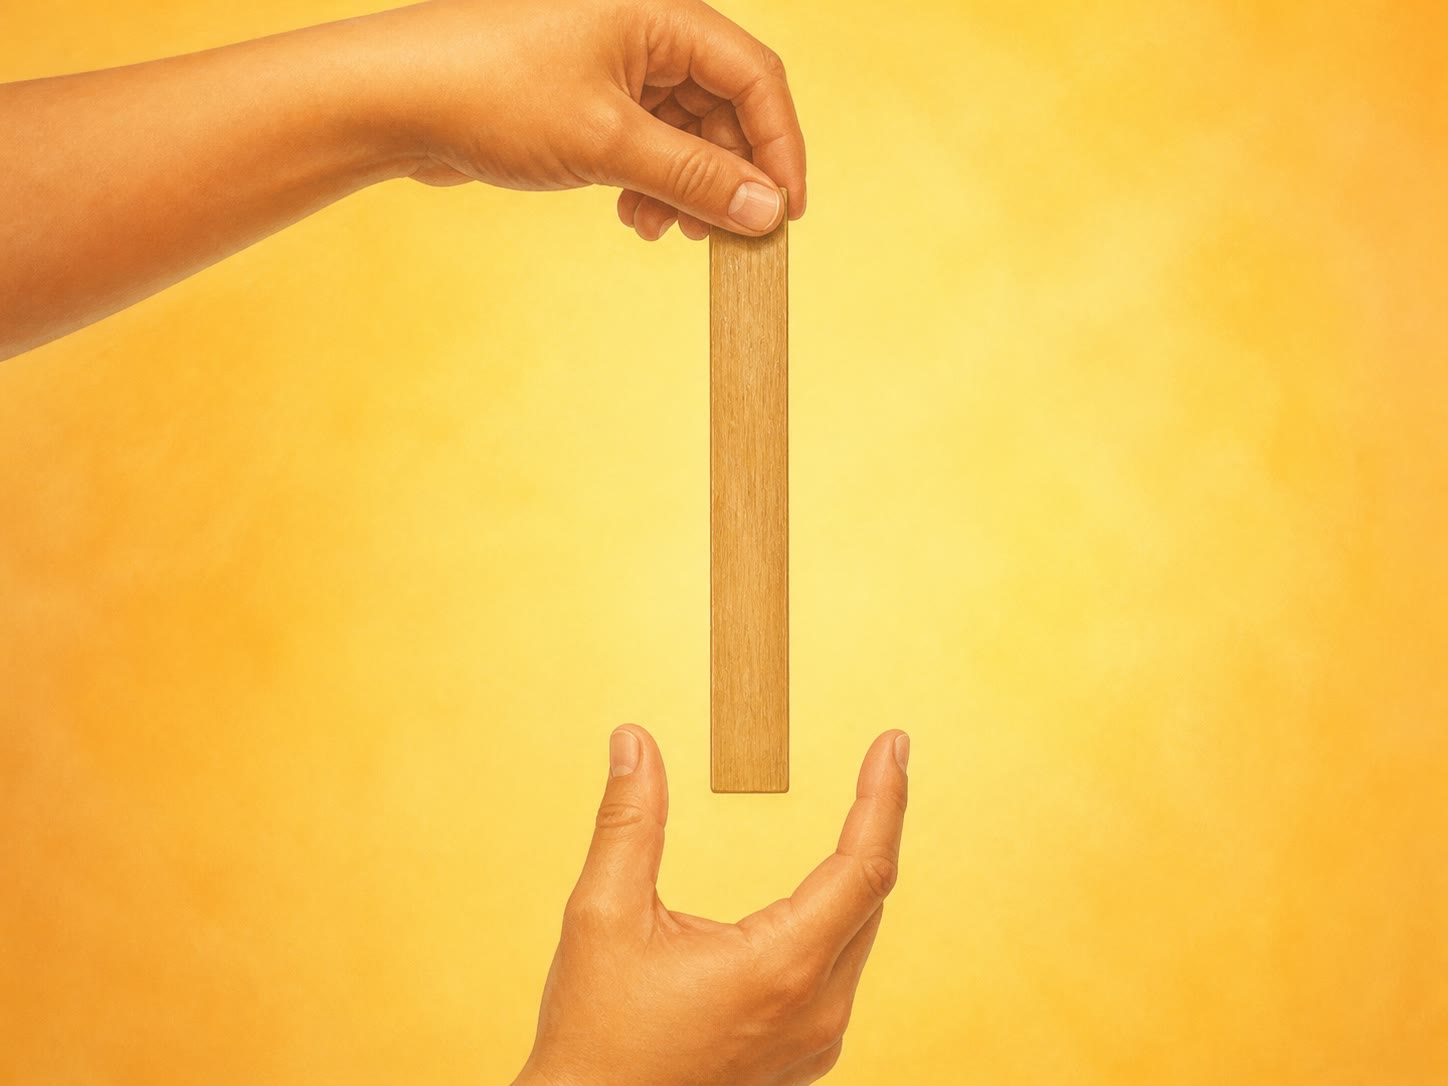
\includegraphics[width=0.5\linewidth]{images/book1/ai/g5-brain-ruler.jpg}

{\small पैमाने वाली जाँच, छोड़ने से एक पल पहले: जैसे ही ऊपर वाला हाथ
छोड़ेगा, नीचे वाले का घेरा --- देखो, तय करो, बंद करो --- अपना पाँचवाँ
हिस्सा सेकंड शुरू कर देगा।}
\end{omfigure}

\begin{example}[बग़ल वाली सीट पहले क्यों चीख़ पड़ती है]\label{ex:g5:brain-in-command:driver}
सेकंड का पाँचवाँ हिस्सा कुछ भी नहीं लगता --- जब तक रफ़्तार उसे गुणा न
कर दे। राजमार्ग की चाल पर एक कार पाँचवें हिस्से भर की प्रतिक्रिया के
दौरान लगभग \qty{7}{m} तय कर लेती है: चालक ने ब्रेक छुआ तक नहीं होता,
और कार एक कक्षा जितनी दूरी पार कर चुकी होती है। \omterm{def:g5:brain-in-command:reaction}{प्रतिक्रिया काल} ही वह
वजह है कि गाड़ियों के बीच दूरी रखी जाती है, और कि चालक का ध्यान ख़ुद
एक सुरक्षा-अंग है।
\end{example}

\begin{remark}[घेरे को साधना]\label{rem:g5:brain-in-command:training}
अभ्यास घेरे को छोटा और पैना कर देता है --- \omterm{def:g5:brain-in-command:system}{तंत्रिकाओं} की रफ़्तार नहीं,
बल्कि \omterm{def:g5:brain-in-command:system}{मस्तिष्क} का रास्ता चुनना। नया बाज़ीगर सब कुछ गिरा देता है; महीने
भर बाद वही \omterm{def:g5:brain-in-command:system}{मस्तिष्क} उन्हीं हाथों को तीन गेंदों में से बिना किसी दिखती
मेहनत के चला देता है। कोई हुनर सीखना \omterm{def:g5:brain-in-command:system}{मस्तिष्क} का बेहतर रास्ते बिछाना है
--- यानी एक और चीज़ जो क़सरत से बढ़ती है, जैसे
\cref{met:g3:bones-and-muscles:care} की \omterm{def:g3:bones-and-muscles:muscle}{पेशियाँ}।
\end{remark}

\section{कमान संभालने वाले की हिफ़ाज़त}

\begin{proposition}[नींद, भोजन, सुरक्षा]\label{prop:g5:brain-in-command:protect}
\omterm{def:g5:brain-in-command:system}{मस्तिष्क} शरीर का सबसे सुरक्षित अंग है --- \omterm{def:g3:bones-and-muscles:skeleton}{खोपड़ी} का टोप, \omterm{def:g4:classifying-animals:vertebrate}{रीढ़} का खंभा
--- और सबसे माँग करने वाला भी: शरीर के वज़न का छोटा-सा हिस्सा होते हुए
भी वह उसकी \omterm{prop:g3:balanced-diet:jobs}{ऊर्जा} और ऑक्सीजन का बड़ा हिस्सा खाता है
(\cref{prop:g4:heart-and-blood:carries}), और अपनी फ़ाइलिंग तथा मरम्मत
\emph{\omterm{prop:g1:healthy-habits:needs}{नींद}} के दौरान करता है
(\cref{prop:g1:healthy-habits:needs})। थका हुआ \omterm{def:g5:brain-in-command:system}{मस्तिष्क} बुरी कमान
चलाता है: धीमी प्रतिक्रियाएँ, बिखरा ध्यान, चिड़चिड़े फ़ैसले।
\end{proposition}
\admitted

\begin{example}[हेलमेट घेरे के लिए हैं]\label{ex:g5:brain-in-command:helmet}
\omterm{def:g3:bones-and-muscles:skeleton}{हड्डियाँ} जुड़ जाती हैं (\cref{rem:g3:bones-and-muscles:alive});
\omterm{def:g5:brain-in-command:system}{मस्तिष्क} का ऊतक, एक बार बुरी तरह चोट खा ले, तो ज़्यादातर नहीं जुड़ता।
साइकिल के हेलमेट के पीछे यही हिसाब है: जहाँ शरीर की अपनी रक्षा शायद
काफ़ी न हो, वहाँ \omterm{def:g3:bones-and-muscles:skeleton}{खोपड़ी} के ऊपर फ़ोम भी। बाक़ी सब चलाने वाले अंग के लिए
यह सस्ता बीमा है।
\end{example}

\section{अभ्यास}

\begin{exercise}[$\star$]\label{exo:g5:brain-in-command:1}
\omterm{def:g5:brain-in-command:system}{तंत्रिका तंत्र} के तीनों भागों के नाम और हर एक की भूमिका बताओ।
\end{exercise}

\begin{exercise}[$\star$]\label{exo:g5:brain-in-command:2}
हर क्रिया का घेरा तीन चरणों में बताओ। कौन ख़बर देता है, कौन फ़ैसला करता
है, और कौन मानता है?
\end{exercise}

\begin{exercise}[$\star$]\label{exo:g5:brain-in-command:3}
\omterm{def:g5:brain-in-command:system}{मस्तिष्क} और \omterm{def:g5:brain-in-command:system}{मेरुरज्जु} कहाँ-कहाँ सुरक्षित रहते हैं, और किन \omterm{def:g3:bones-and-muscles:skeleton}{हड्डियों}
से?
\end{exercise}

\begin{exercise}[$\star$]\label{exo:g5:brain-in-command:4}
\omterm{def:g5:brain-in-command:reaction}{प्रतिक्रिया काल} क्या है? किसी सरल काम के लिए उसका मोटा मान बताओ।
\end{exercise}

\begin{exercise}[$\star$]\label{exo:g5:brain-in-command:5}
\cref{ex:g5:brain-in-command:catch} की तरह धीरे-धीरे दोहराओ: तुम किसी
नुकीली चीज़ पर पैर रख देते हो और तुम्हारा पैर झटके से हट जाता है।
ख़बर किसने दी, फ़ैसला किसने किया, और माना किसने?
\end{exercise}

\begin{exercise}[$\star$]\label{exo:g5:brain-in-command:6}
\cref{rem:g5:brain-in-command:more} से दो ऐसी सेवाएँ बताओ जो \omterm{def:g5:brain-in-command:system}{मस्तिष्क}
तुम्हारे सोचे बिना ही चलाता है।
\end{exercise}

\begin{exercise}[$\star$]\label{exo:g5:brain-in-command:7}
थका हुआ \omterm{def:g5:brain-in-command:system}{मस्तिष्क} बुरी कमान क्यों चलाता है?
\cref{prop:g5:brain-in-command:protect} से उसकी दो ज़रूरतें बताओ।
\end{exercise}

\begin{exercise}[$\star$]\label{exo:g5:brain-in-command:8}
करके देखो: \cref{met:g5:brain-in-command:ruler} वाली पैमाने की जाँच
पाँच बार चलाओ। अपनी आम पकड़-दूरी बताओ --- और यह भी कि अभ्यास से उसमें
सुधार हुआ या नहीं।
\end{exercise}

\begin{exercise}[$\star\star$]\label{exo:g5:brain-in-command:9}
चाहे लपकने वाला कितना ही कुशल हो, तत्काल लपक जैसी कोई चीज़ क्यों नहीं
होती? घेरे के तीनों चरणों से उत्तर दो।
\end{exercise}

\begin{exercise}[$\star\star$]\label{exo:g5:brain-in-command:10}
\cref{ex:g5:brain-in-command:driver} की मदद से: सड़क के नियम अच्छे
ब्रेकों भर के बजाय गाड़ियों के बीच \emph{दूरी} की माँग क्यों करते हैं?
ध्यान घेरे में क्या बदल देता है?
\end{exercise}

\begin{exercise}[$\star\star\star$]\label{exo:g5:brain-in-command:11}
\cref{rem:g5:brain-in-command:training} की बाज़ीगर बेहतर हुई, जबकि
उसकी \omterm{def:g5:brain-in-command:system}{तंत्रिकाएँ} ज़रा भी तेज़ नहीं हुईं। इसके बजाय घेरे का कौन-सा हिस्सा
बेहतर हुआ? \omterm{def:g3:bones-and-muscles:muscle}{पेशी} को साधने से तुलना करो: हर हाल में बढ़ता क्या है?
\end{exercise}
